%\documentstyle[a4j,epsbox,graphicx]{jarticle}
\documentclass[a4j]{jarticle}%変更禁止!
%%%%%%%%%%%%usepackageは適宜追加してください.%%%%%%%%%%%%%%%%%%%%%%%%%%%%%%%%%%%%%%%%%%%%%%%%%%%
%\usepackage{epsbox}
%\usepackage{graphicx}
\usepackage[dvipdfmx]{graphicx,color}
%%%%%%%%%%%%%%%%%%%%%%%%%%%ここから変更禁止%%%%%%%%%%%%%%%%%%%%%%%%%%%%%%%%%%%%%%%%%%%%%%%%%%
\topmargin -28mm
\oddsidemargin -15mm
\evensidemargin -15mm
\textwidth 185mm
\textheight 275mm
\columnsep 6mm

%\def\toujitu{Dec. 2020}

\makeatletter
\def\section{\@startsection{section}{2}{\z@}{.8ex plus .8ex minus 
 .2ex}{.05ex plus .07ex}{\large\bf}}
\makeatother
\makeatletter
\def\subsection{\@startsection{subsection}{2}{\z@}{.8ex plus .8ex minus 
 .2ex}{.05ex plus .07ex}{\bf}}
\makeatother


\pagestyle{empty}

\begin{document}

\baselineskip 4.75mm

\twocolumn
[
  \footnotesize
  \begin{center}
    {~}\\
    %\begin{center}
    %{ユビキタスウェアラブルワークショップ2020 
    %\hfill \toujitu}\\
    %%%%%%%%%%%%%%%%%%%%%%%%%%%ここまで変更禁止%%%%%%%%%%%%%%%%%%%%%%%%%%%%%%%%%%%%%%%%%%%%%%%%%%

    %%%注意!!\vspaceは図表部分のみ見にくく(醜く)ならない範囲内で使用可能とします.%%%%%%%%%%%%%%%%%%%%%%%%%%%%

    \medskip
    {\large
      %タイトル
      {\bf ディスプレイを用いた擬似的脈波生成手法の検討}\\
    }
    \medskip
    {\large
      %著者 同じ所属の人が連続する場合は連続する同じ所属の著者の最後の著者のみに所属を付けること.
      藤井敦寛(立命館大学),村尾和哉(立命館大学,JSTさきがけ)
    }
  \end{center}
]

\section{研究の背景と目的}
近年,健康管理への意識の高まりから,自身の生体情報を記録するウェアラブルデバイスが広く普及してきている.記録する生体情報は活動量や呼吸数,体温など様々な情報があり,心拍数もその一つである.心拍数を取得するために用いられる脈波センサでは,緑色のLEDを皮膚に照射して,反射した光の変化から脈波を計測する光電式容積脈波記録法(PPG)と呼ばれる方式のものが一般的であり,スマートウォッチなどにも導入されている.しかしながら,皮膚内の血管に向けて光を照射するという特性上,センサの装着位置に血管が存在しない場合は使用が不可能である.例えば,義手にスマートウォッチを装着する場合,正常な心拍数は取得できない.

そこで我々は,他の身体部位から取得した脈波データを用いて,擬似的に脈波値を生成する手法を検討する.

本研究ではパルスセンサーを用いる.これは,緑色反射方式を使用した脈波センサの一つであり,広く普及してきている環境を再現できる.

\section{これまでの研究内容}
本章では,これまでのUWWの歴史について述べる.

UWWは,大学と企業の間の垣根を取り払い,ユビキタスウェアラブルの未来について語り合い,学生間の交流を深めるために開催された.本ワークショップは,2007年にシーサイドホテル舞子ビラ神戸で行われた第1回より,神戸市(2008, 2010, 2016),三木市(2009),舞子市(2011, 2012),淡路市(2013--2019)と兵庫県内各地の会場で開催され,今年で14回目となる.UWWでは,出席者全員でワークショップを盛り上げることを原則としており,この伝統は今も代々受け継がれている.第1回の発表者は47人,プロシーディングは48ページだった.

ここでは,昨年行われたUWW2019\cite{bib1}について述べる.UWW2019の表紙を図\ref{fig1}に示す.この年は,2日間で計70人が濃密な発表を行った.学生は緊張した面持ちで発表を行い,企業の方はウェアラブル技術の最新動向について報告を行い,先生方は研究者として,ユビキタスウェアラブルの将来を熱く語った.すべての参加者がユビキタスウェアラブルに対する情熱をぶつけ合った発表会は,数多くの驚きと笑いを巻き起こし,閉幕した.

また,神戸ルミナリエの開催中に行われた第4回以外のUWWはすべて合宿形式で行われた.詳細は諸々の事情で今回もやはり言及しないが,学生たちは新たな知見に出会い,親睦を深めた.

\section{オリジナルバーガーの作り方(昔の話)}
\begin{itemize}
  \item マクドで65円ハンバーガー3個をテイクアウト.
  \item 飲み物は大型スーパーの1個38円ジュース.
  \item オカンが揚げた冷凍ポテトとチキンナゲットをバーガーに挟む.
  \item オカンが準備したレタスとケチャップで彩り,完成.
\end{itemize}

表\ref{table1}のように表を作成してもよい.

\begin{figure}[!t]
  \begin{center}
    \includegraphics[width=0.8\linewidth]{fig1.eps}
  \end{center}
  \vspace{-8mm}
  \caption{ユビキタスウェアラブルワークショップ2019表紙}%{}内にタイトルを記入してください
  \label{fig1}
\end{figure}

%論文の理解を助けるための図表を適宜入れること.

\section{おわりに}
本研究では,UWWの成果を記録に残し,当日の発表内容を手軽に理解するために,統一的な論文形式を提案し,実装を行った.また,これまでのUWWの歴史を紹介し,UWWで今後生まれる予定の黒歴史の一端を暗示した.

今後の予定は,UWWのプロシーディングで本フォーマットを使用していただき,UWWの発表で活発な議論が行われることを妄想し,UWWの発展を祈念することである\cite{bib2,bib9,bib10,bib11,bib12,bib13,bib14,bib15}.

\begin{table}[h]
  \begin{center}
    \caption{上新先生のトキメキモーニングルーティン}
    \label{table1}
    \begin{tabular}{c|l}\hline\hline
      時間帯 & 行動                                   \\\hline
      起床後 & コップ一杯の常温水で鼻うがい.         \\
      朝食   & 新鮮なフルーツ.オススメはドリアン.   \\
      出勤前 & 昼ご飯の献立と一日サボる方法を考える. \\\hline
    \end{tabular}
  \end{center}
\end{table}

\begin{thebibliography}{10}

  \bibitem{bib1} ユビキタスウェアラブルワークショップ2019プロシーディング (2019).
  \bibitem{bib2} Buruo, U., and Tasumi, Y.: New Wearable Generation, Trans. Ubi. Wearable, Vol. 7, No. 7, pp. 77-88 (2000).
  % \bibitem{bib3} 上新振留夫,指木多須美:ウェアラブル環境における HMD を用いたすれ違い出会い通信システムの設計と実装,穂下穂下処理学会論文誌,Vol. 38, No. 2, pp. 111-123 (2009).
  % \bibitem{bib4} 上新振留夫,指木多須美:ウェアラブル環境における HMD を用いた残り寿命表示システムの実現,穂下穂下処理学会論文誌,Vol. 40, No. 1, pp. 11-20 (2011).
  % \bibitem{bib5} 上新振留夫:ウェアラブルよ,永遠なれ,骨川書房 (2008).
  % \bibitem{bib6} 上新振留夫:ウェアラブル,お前もか,骨川書房 (2010).
  % \bibitem{bib7} 上新振留夫:部屋とウェアラブルと私,骨川書房 (2012).
  % \bibitem{bib8} 上新振留夫,指木多須美:ウェアラブル環境における HMD を用いた高齢者向けバーチャル恋愛システム「ゲートボールで攻めて恋」の実現,穂下穂下処理学会論文誌,Vol. 42, No. 2, pp. 25-32 (2013).
  \bibitem{bib9} 上新振留夫:ウェアラブル川柳$\sim$キ(着)テる貴方に送る,17文字のメッセージ$\sim$,骨川書房 (2014).
  \bibitem{bib10} 指木多須美:ドローンを利用した町内スーパーの特売情報リアルタイム取得システム,穂下穂下処理学会論文誌,Vol. 44, No. 3, pp. 58-65 (2015).
  \bibitem{bib11} 上新振留夫:UWW十年史,骨川ファンタジア文庫 (2016).
  \bibitem{bib12} 指木多須美,上新振留夫:ユーザの無意識動作に基づくウェアラブル端末の暗号化方式の提案,穂下穂下処理学会論文誌,Vol. 46, No. 9, pp. 179-187 (2017).
  \bibitem{bib13} 上新振留夫:ウェアラブルを止めるな!,骨川ファンタスティック映画祭正式出品,上新フィルムパートナーズ (2018).
  \bibitem{bib14} 指木多須美,上新振留夫:幼児の行動様式に基づくウェアラブル端末を用いたオートパイロット育児システムの提案,穂下穂下処理学会論文誌,Vol. 48, No. 5, pp. 80-88 (2019).
  \bibitem{bib15} 上新振留夫,指木多須美:特殊刀による必殺技習得のためのウェアラブル端末を用いた剣道学習支援システムの提案,穂下穂下処理学会論文誌,Vol. 49, No. 6, pp. 60-68 (2020).
\end{thebibliography}
\end{document}